% Copyright 2004 by Till Tantau <tantau@users.sourceforge.net>.
%
% In principle, this file can be redistributed and/or modified under
% the terms of the GNU Public License, version 2.
%
% However, this file is supposed to be a template to be modified
% for your own needs. For this reason, if you use this file as a
% template and not specifically distribute it as part of a another
% package/program, I grant the extra permission to freely copy and
% modify this file as you see fit and even to delete this copyright
% notice. 

\documentclass{beamer}

% There are many different themes available for Beamer. A comprehensive
% list with examples is given here:
% http://deic.uab.es/~iblanes/beamer_gallery/index_by_theme.html
% You can uncomment the themes below if you would like to use a different
% one:
%\usetheme{AnnArbor}
%\usetheme{Antibes}
%\usetheme{Bergen}
%\usetheme{Berkeley}
%\usetheme{Berlin}
%\usetheme{Boadilla}
%\usetheme{boxes}
%\usetheme{CambridgeUS}
%\usetheme{Copenhagen}
%\usetheme{Darmstadt}
%\usetheme{default}
%\usetheme{Frankfurt}
%\usetheme{Goettingen}
%\usetheme{Hannover}
%\usetheme{Ilmenau}
%\usetheme{JuanLesPins}
%\usetheme{Luebeck}
%\usetheme{Malmoe}
%\usetheme{Marburg}
%\usetheme{Montpellier}
%\usetheme{PaloAlto}
%\usetheme{Pittsburgh}
%\usetheme{Rochester}
%\usetheme{Singapore}
%\usetheme{Szeged}
%\usetheme{Warsaw}


\usetheme{Madrid}


\usepackage{xcolor}
\usepackage{comment}
\usepackage{listings}
\usepackage{color}
\usepackage{courier}

\definecolor{lightgray}{rgb}{.9,.9,.9}
\definecolor{darkgray}{rgb}{.4,.4,.4}
\definecolor{purple}{rgb}{0.65, 0.12, 0.82}

\lstdefinelanguage{JavaScript}{
  keywords={typeof, new, true, false, catch, function, return, null, catch, switch, var, if, in, while, do, else, case, break},
  keywordstyle=\color{blue}\bfseries,
  ndkeywords={class, export, boolean, throw, implements, import, this},
  ndkeywordstyle=\color{darkgray}\bfseries,
  identifierstyle=\color{black},
  sensitive=false,
  comment=[l]{//},
  morecomment=[s]{/*}{*/},
  commentstyle=\color{purple}\ttfamily,
  stringstyle=\color{red}\ttfamily,
  morestring=[b]',
  morestring=[b]"
}

\lstset{
   language=JavaScript,
   %backgroundcolor=\color{lightgray},
   extendedchars=true,
   basicstyle=\footnotesize\ttfamily,
   showstringspaces=false,
   showspaces=false,
   showtabs=true,
   %numbers=left,
   %numberstyle=\footnotesize,
   %numbersep=9pt,
   tabsize=2,
   breaklines=true,
   showtabs=false,
   captionpos=b
}

\definecolor{light-gray}{gray}{0.75}
\newcommand{\light}[1]{\textcolor{light-gray}{#1}}


\title{Structural Design Patterns}

% A subtitle is optional and this may be deleted
\subtitle{Motivation and Examples}

\author{Ahmed Khattab}
% - Give the names in the same order as the appear in the paper.
% - Use the \inst{?} command only if the authors have different
%   affiliation.

\institute[TUM]{Technische Universit{\"a}t M{\"u}nchen}
% (optional, but mostly needed)

% - Use the \inst command only if there are several affiliations.
% - Keep it simple, no one is interested in your street address.

\date[28.04.2015]{Patterns and Anti-Patterns, 28th of April 2015}
% - Either use conference name or its abbreviation.
% - Not really informative to the audience, more for people (including
%   yourself) who are reading the slides online

%\subject{Theoretical Computer Science}
% This is only inserted into the PDF information catalog. Can be left
% out. 

% If you have a file called "university-logo-filename.xxx", where xxx
% is a graphic format that can be processed by latex or pdflatex,
% resp., then you can add a logo as follows:

% \pgfdeclareimage[height=0.5cm]{university-logo}{university-logo-filename}
% \logo{\pgfuseimage{university-logo}}

% Delete this, if you do not want the table of contents to pop up at
% the beginning of each subsection:
\AtBeginSubsection[]
{
  \begin{frame}<beamer>{Outline}
    \tableofcontents[currentsection,currentsubsection]
  \end{frame}
}

% Let's get started
\begin{document}

\begin{frame}
  \titlepage
\end{frame}

\begin{frame}{Outline}
  \tableofcontents
  % You might wish to add the option [pausesections]
\end{frame}

% Section and subsections will appear in the presentation overview
% and table of contents.
\section{Definition And Motivation}

\begin{frame}{Structural Patterns}%{Optional Subtitle}
 \begin{block}{Definition}
 \begin{itemize}
   \item {Concerned with how object are composed to form more complex structures}
   \item {Provide simple ways to realize relationships between objects}
 \end{itemize}
 \end{block}
 
 \begin{block}{Motivation}
 \begin{itemize}
   \item {Flexibility to change}
   \item {Extensibility}
   \item {Structured code reuse}
 \end{itemize}
 \end{block}
\end{frame}

\section{Examples of structural patterns}

% You can reveal the parts of a slide one at a time
% with the \pause command:
\begin{frame}{Examples of structural patterns}
  \begin{itemize}
   \item {
    Adapter Pattern
  }
  \item {   
    Composite Pattern
  }
  % You can also specify when the content should appear
  % by using <n->:
  \item {
    Decorator Pattern
  }
  \item {
    Bridge Pattern
  }
  \item {
    Fa\c{c}ade Pattern
  }
  \item {
    Flyweight Pattern
  }
  \item {
    Proxy Pattern
  }
  \item {
    Aggregate Pattern
    %\pause % The slide will pause after showing the first item
  }
   \item {
    ...
  }
  % or you can use the \uncover command to reveal general
  % content (not just \items):
  \end{itemize}
\end{frame}

\begin{frame}{Our focus}
Our focus will be on:
  \begin{itemize}

  \item {
    \light{Adapter Pattern}
  }
  \item {   
    \light{Composite Pattern}
  }
  % You can also specify when the content should appear
  % by using <n->:
  \item {
    Decorator Pattern
  }
  \item {
    \light{Bridge Pattern}
  }
  \item {
    Fa\c{c}ade Pattern
  }
  \item {
    \light{Flyweight Pattern}
  }
   \item {
    Proxy Pattern
  }
  \item {
    \light{Aggregate Pattern}
    %\pause % The slide will pause after showing the first item
  }
   \item {
    ...
  }
  % or you can use the \uncover command to reveal general
  % content (not just \items):
  \end{itemize}
\end{frame}


\subsection{Proxy Pattern}
\begin{frame}{Proxy Pattern}
  \begin{block}{Definition}
   \begin{itemize}
    \item { Sits between the client of an object and the object itself }
    \item { Controls access to the object }
   \end{itemize}
  \end{block}
  \pause
  \begin{block}{Common Scenarios}
   \begin{itemize}
    \item { Controlling the instantiation of an expensive object }
    \item { Making a remote object seem local }
    \item { Caching (web service requests, rendering of graphical elements, ... }
   \end{itemize}
  \end{block}
\end{frame}

\begin{frame}{Proxy Pattern - The analogy}
 \begin{figure}[htp]
    \centering
    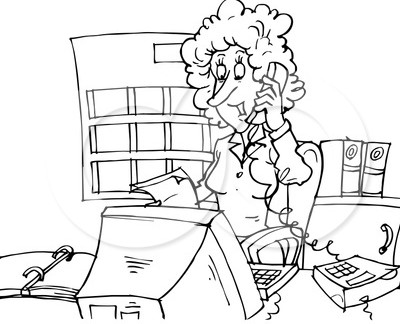
\includegraphics[width=7cm]{pics/secretary}
    \label{fig:proxy}
    \end{figure}
\end{frame}

\begin{frame}{Proxy Pattern - In Detail}
    \begin{figure}[htp]
    \centering
    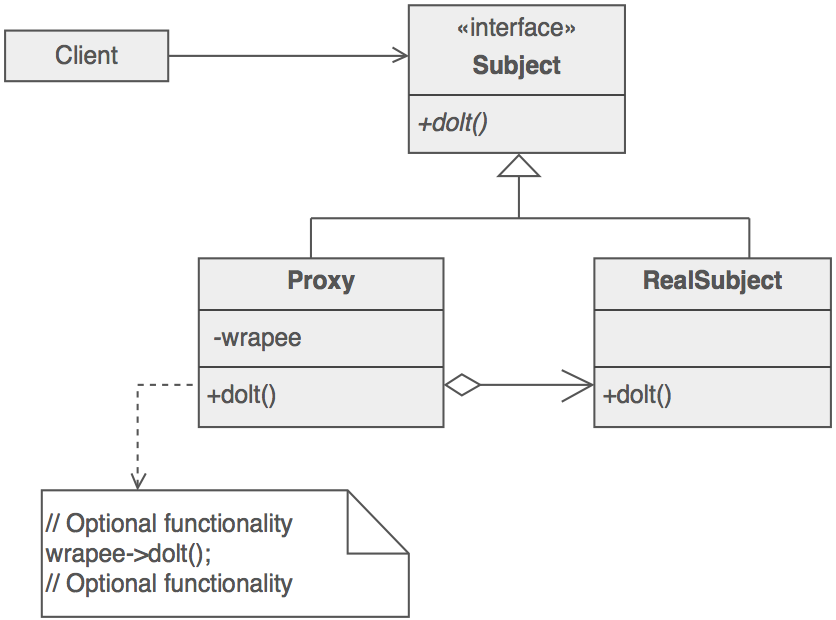
\includegraphics[width=7cm]{pics/proxy2}
    \label{fig:proxy2}
    \end{figure}
\end{frame}


\subsection{Decorator Pattern}
\begin{frame}{Decorator Pattern}
  \begin{block}{Definition}
   \begin{itemize}
    \item {Allowing the addition of functionality to an object dynamically}
    \item {Provide a flexible alternative to subclassing for extending functionality}
   \end{itemize}
  \end{block}
  \pause
  \begin{block}{Common Scenarios}
   \begin{itemize}
    \item { Adding additional features to objects without heavily modifying the code using them}
    \item { Too many dynamic options that can be added, making subclassing a headache }
    \item { e.g. Lord of the rings game, different roles (elf, orc, hobbit, etc..) }
   \end{itemize}
  \end{block}
\end{frame}


\begin{frame}{Decorator Pattern - The analogy}
    \begin{figure}[htp]
    \centering
    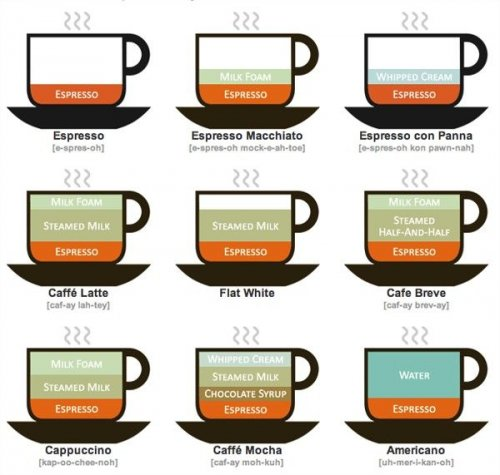
\includegraphics[width=6cm]{pics/coffee}
    \label{fig:decorator}
    \end{figure}
\end{frame}

\begin{frame}{Decorator Pattern - In Detail}
    \begin{figure}[htp]
    \centering
    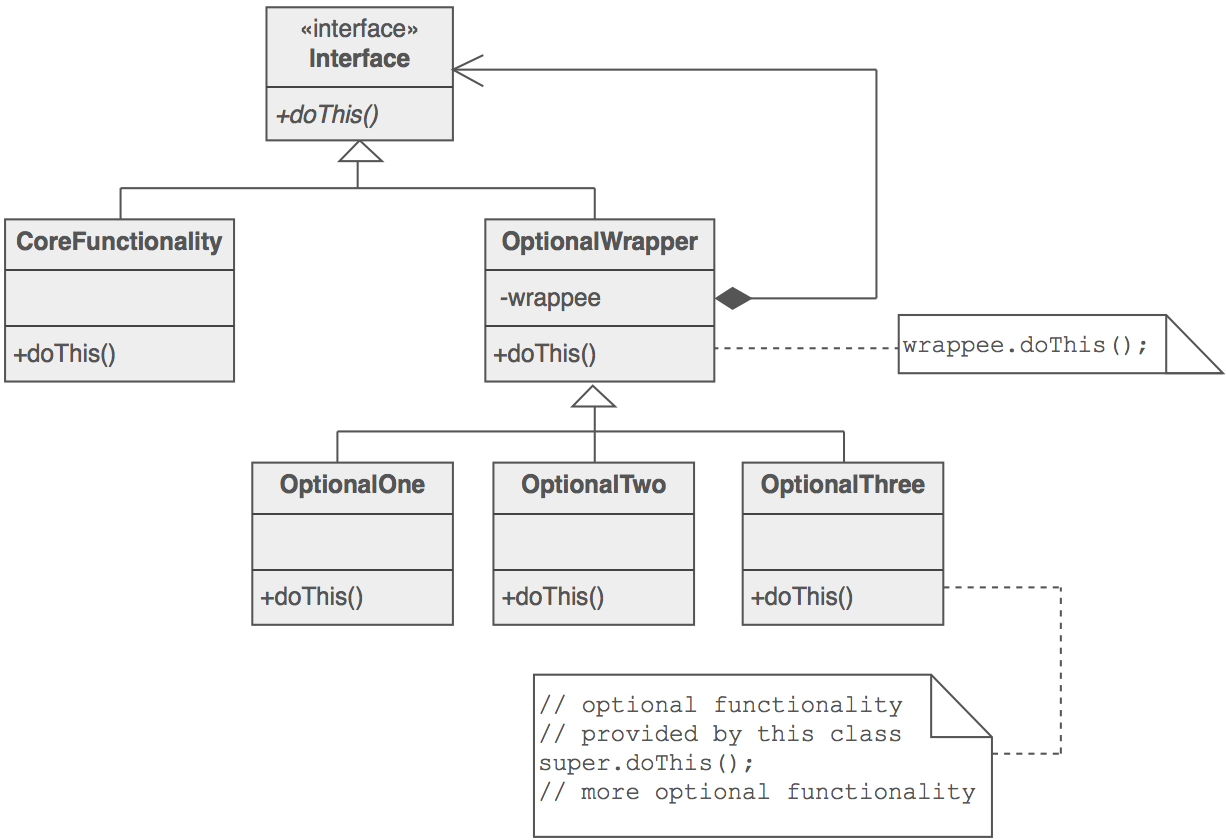
\includegraphics[width=8cm]{pics/decorator2}
    \label{fig:decorator2}
    \end{figure}
\end{frame}

\subsection{Fa\c{c}ade Pattern}
\begin{frame}{Fa\c{c}ade Pattern}
  \begin{block}{Definition}
   \begin{itemize}
    \item {Provides a simpler abstracted interface to a larger (potentially more complex) body of code.}
   \end{itemize}
  \end{block}
  \pause
  \begin{block}{Common Scenarios}
   \begin{itemize}
    \item { Interface to abstract access to several complex subsystems }
    \item { Wrap a poorly designed collection of APIs with a single well-designed API }
   \end{itemize}
  \end{block}
\end{frame}

\begin{frame}{Fa\c{c}ade Pattern - The analogy}
    \begin{figure}[htp]
    \centering
    
\includegraphics[width=7cm]{pics/facade2}
    \label{fig:facade}
    \end{figure}
\end{frame}


\begin{frame}{Fa\c{c}ade Pattern - In Detail}
    \begin{figure}[htp]
    \centering
    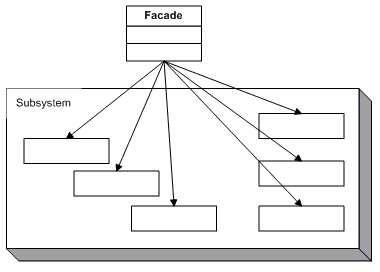
\includegraphics[width=7cm]{pics/facade}
    \label{fig:facade2}
    \end{figure}
\end{frame}

\section{Structural patterns in action}
\subsection{The Weather App}

 \begin{frame}{The Weather App}
A simple application for fetching location-specific weather information from a web service
    \begin{figure}[htp]
    \centering
    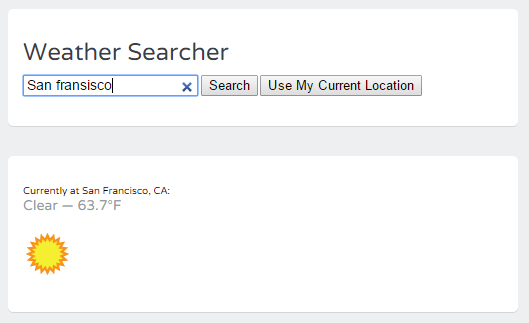
\includegraphics[width=6cm]{pics/weathersearcher2}
    \label{fig:weather1}
    \end{figure}
\end{frame}

 \begin{frame}{The Weather App}
Upon no location match: a list of suggested locations is returned
    \begin{figure}[htp]
    \centering
    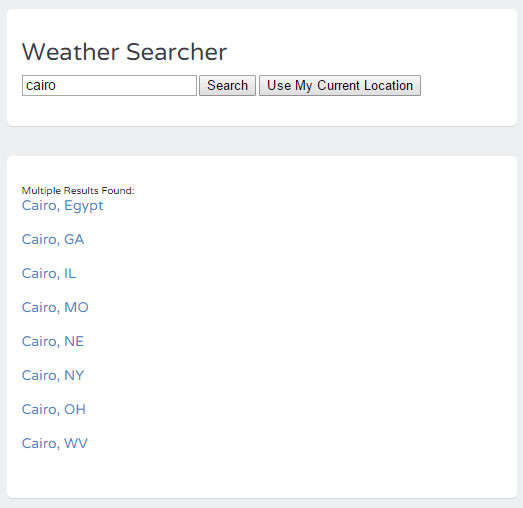
\includegraphics[width=6cm]{pics/weathersearcher}
    \label{fig:weather2}
    \end{figure}
\end{frame}

 \begin{frame}{The Weather App}
The flow:
    \begin{figure}[htp]
    \centering
    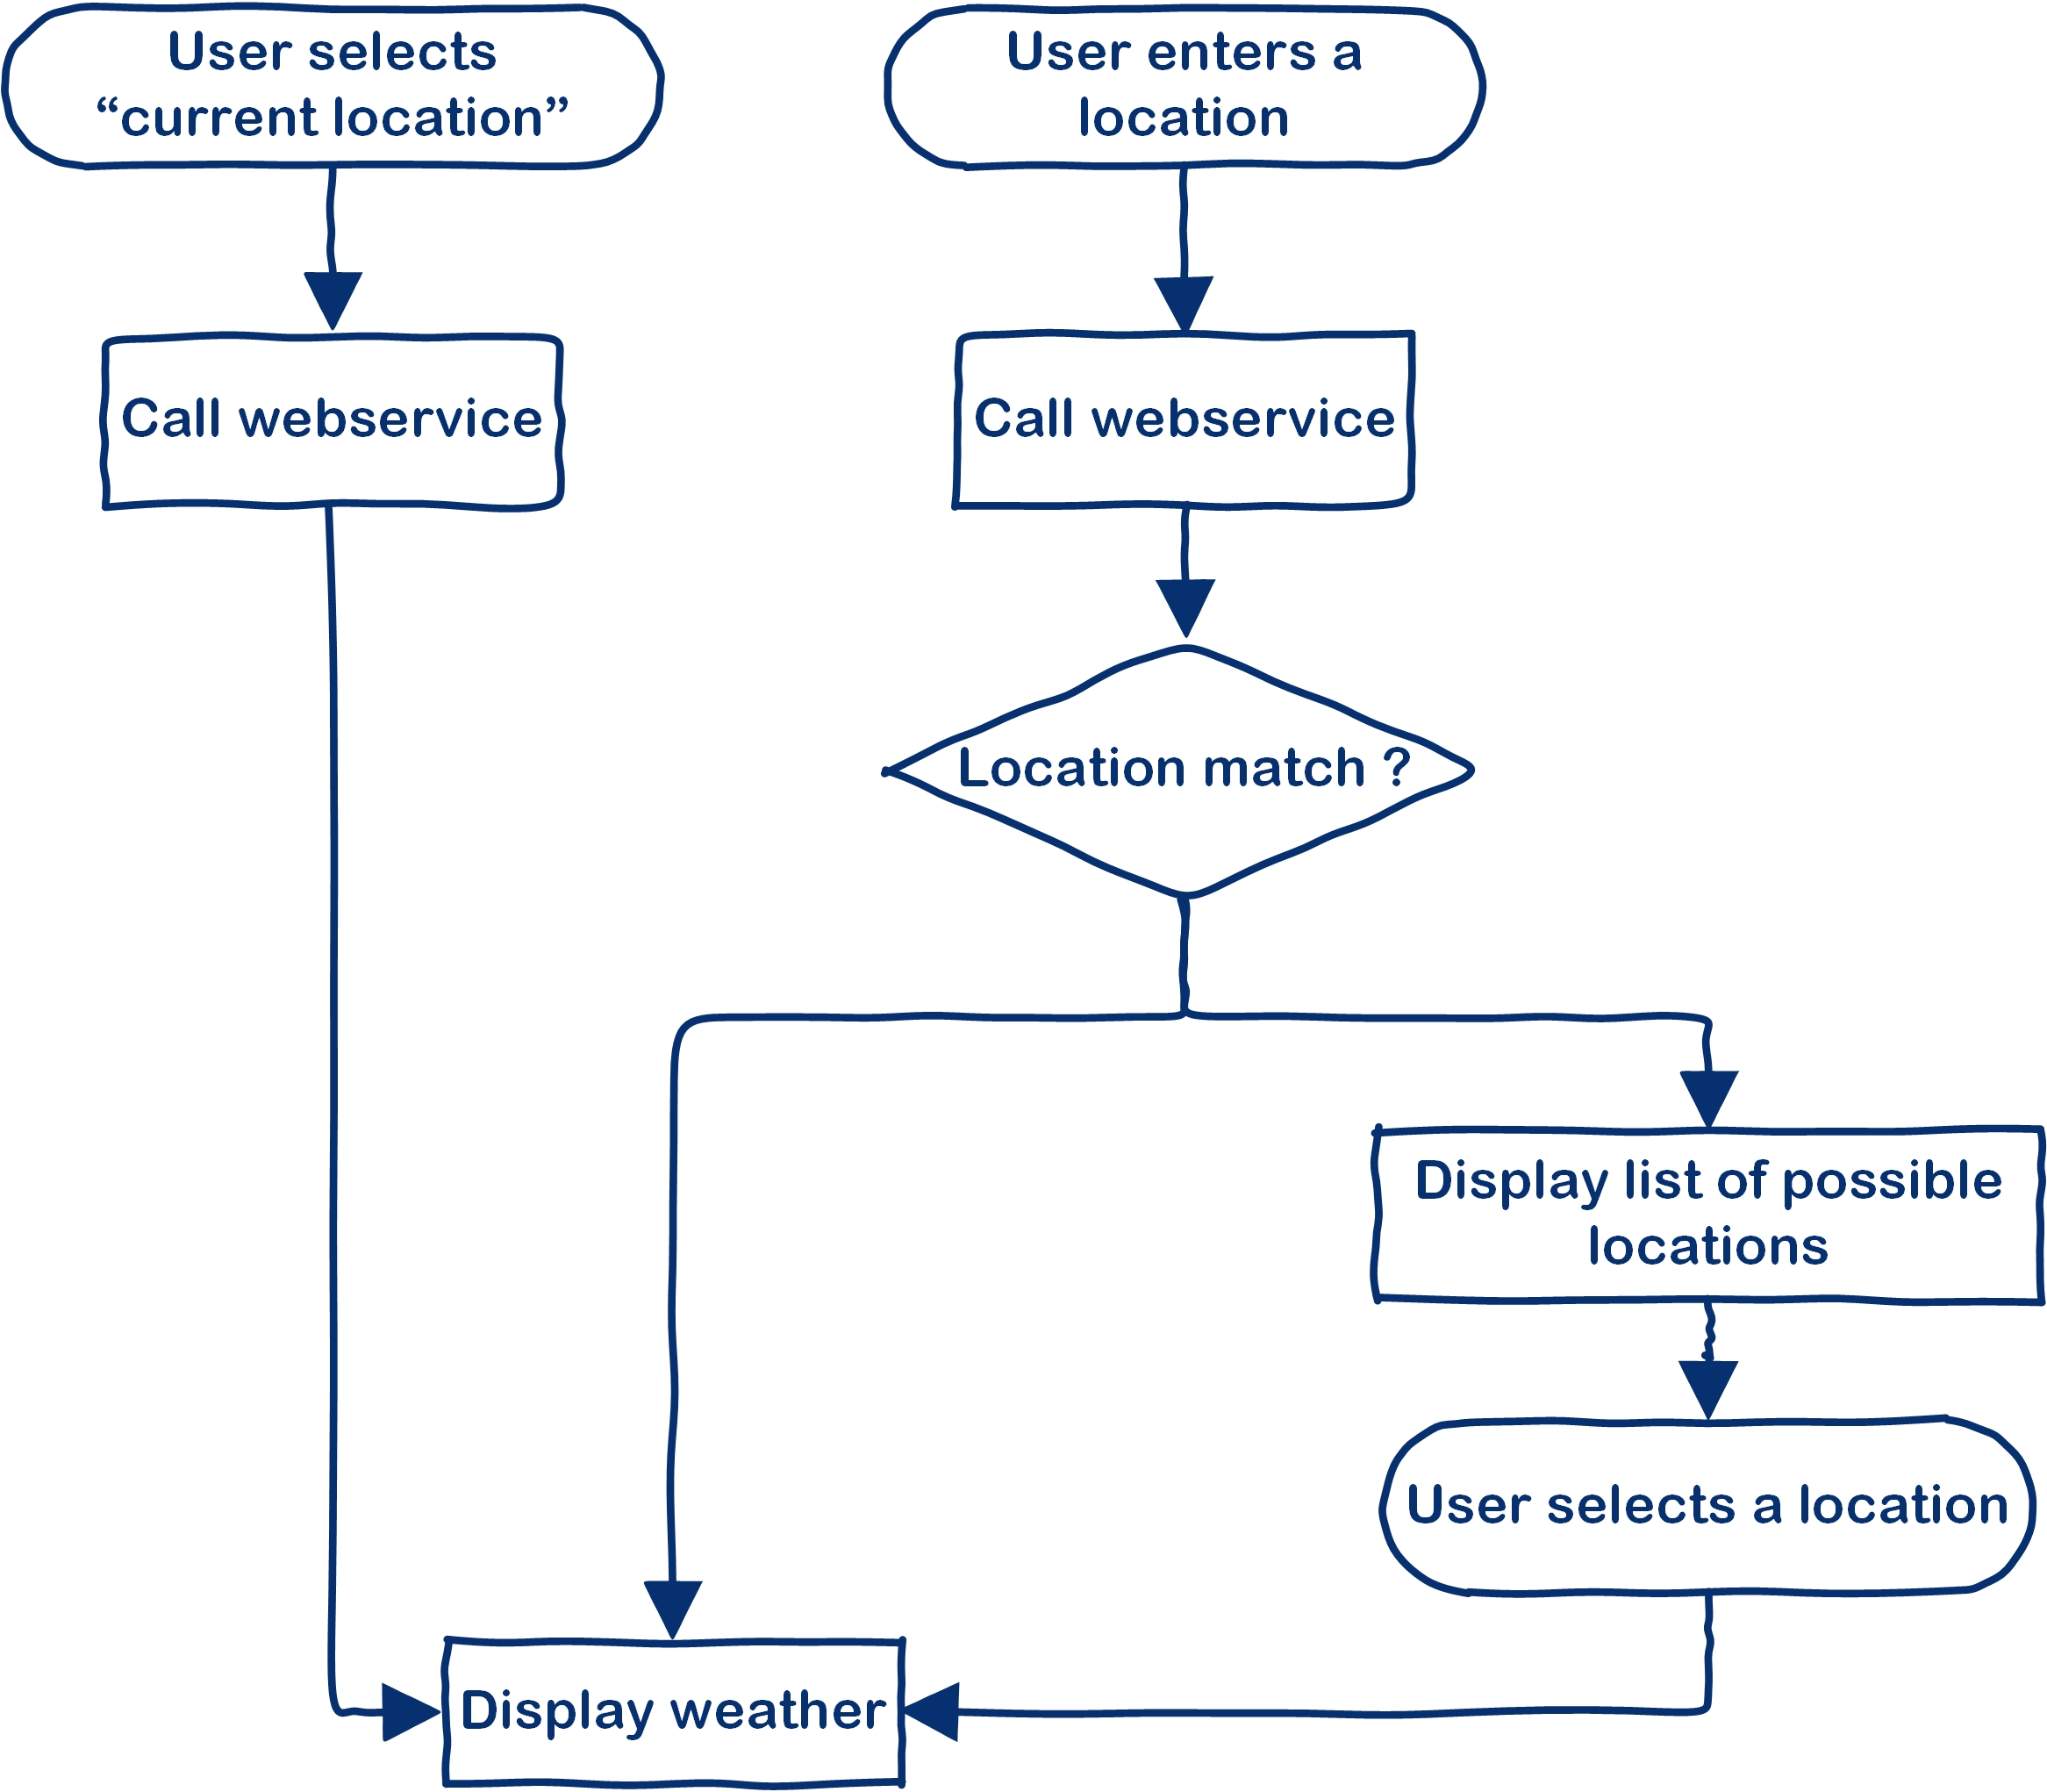
\includegraphics[width=7cm]{pics/weatherapp}
    \label{fig:weather}
    \end{figure}
\end{frame}

\begin{frame}{The Weather App - analysis}
The callback function handles everything
    \begin{itemize}
      \item Receiving response from webservice calls
      \item Parses and displaying weather info when available
      \item Otherwise displays list of possible locations and attaches event handlers for the displayed list
    \end{itemize}
    \begin{block}{Disadvantages}
      \begin{itemize}
    \item Tight coupling between view and control (handling web service calls and rendering of the output in one place)
    \item Suggestions for locations are fetched and the whole list is rendered every time from the web service (Caching ?)
    \end{itemize}
    \end{block}
\end{frame}

\begin{frame}[fragile]
\frametitle{The Weather App - refactoring I}
\textbf{The proxy:}
\begin{lstlisting}
function API() {
	  this.cache = {};
	  
	  this.addToCache = function(location, data){
		  this.cache[location] = data; 
	  }
	  this.searchLocation = function(searchLocation, callback){
		  if(this.cache[searchLocation])
		     // cache hit, load from cache
		  else
		     // cache miss, call web service
	  }
	  this.getWeatherByID = function(searchID, callback){
		  var url = " ... ";
        ...
\end{lstlisting}
\end{frame}

\begin{frame}{The Weather App - refactoring I}
\textbf{The proxy: a class API that provides the following:}
   \begin{itemize}
    \item Encapsulates actual calls to the web service
    \item Manages the cache for caching the returned lists of locations
    \end{itemize}
\end{frame}

\begin{frame}[fragile]
\frametitle{The Weather App - refactoring II}
\textbf{The decorator:}
\begin{lstlisting}
//declare the different decorators
decorators = {};
decorators.locationsResponse = {
   render: function(data){
		//do custom rendering for locations suggestions list...
	  }};
	  
...

var weatherResponse = new BasicResponse(data); 
if(data.locations != '') {
    weatherResponse.decorate('locationsResponse');
}
weatherResponse.render();

\end{lstlisting}
\end{frame}

\begin{frame}[fragile]
\frametitle{The Weather App - refactoring II}
\textbf{The decorator:}
\begin{lstlisting}

function BasicResponse(data) {

	  this.decorator;

	  this.render = function(){
		  var resultHTML;
		  if(this.decorator)
			// a decorator exists, use it to render
			decorators[this.decorator].render(this.data);
		  else {
			// no decorators added, render normally...
	} } }

\end{lstlisting}
\end{frame}

\begin{frame}{The Weather App - refactoring II}
\textbf{The BasicResponse class provides the following:}
\begin{itemize}
    \item An object oriented representation for each response from the web service
    \item A render method to parse and display normal responses
    \item The render method can be decorated to display special responses differently 
\end{itemize}
\end{frame}



\subsection{Pacman}
\begin{frame}{Pacman}
The famous Pacman implemented in JavaScript and HTML5 canvas
    \begin{figure}[htp]
    \centering
    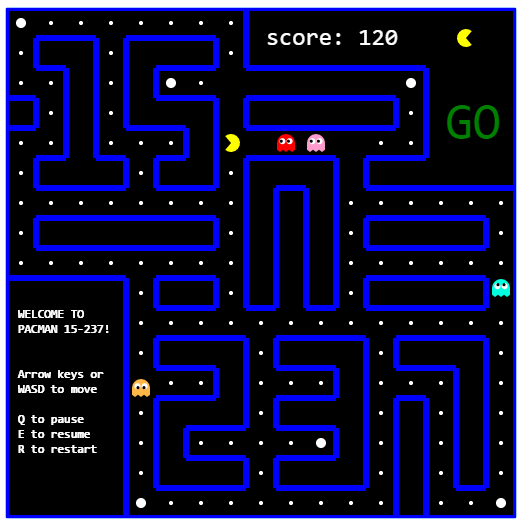
\includegraphics[width=5cm]{pics/pacman}
    \label{fig:pacman}
    \end{figure}
    
\end{frame}

\begin{frame}{Pacman - ghosts.js}
\begin{itemize}
\item Script responsible for representing the Ghost object
\item Handles rendering of the object using HTML5 canvas methods
\item Every ghost can take different forms (color, eye position, ...)
\end{itemize}

    \begin{figure}[htp]
    \centering
    
\includegraphics[width=7cm]{pics/ghosts}
    \label{fig:ghosts}
    \end{figure}
\end{frame}

\begin{frame}{Pacman - analysis}
A huge Ghost.draw() function:
 \begin{itemize}
      \item Checks the status of the ghost (weak or strong, moving or not, ..)
      \item Draws every detail (the eyes, mouth, legs, ...)
    \end{itemize}
   \begin{figure}[htp]
    \centering
    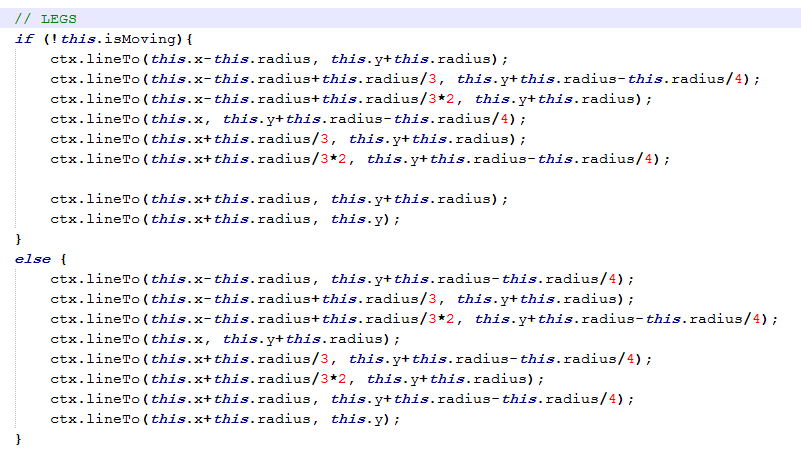
\includegraphics[width=8cm]{pics/Legs}
    \label{fig:legs}
    \end{figure}
\end{frame}

\begin{frame}{Pacman - analysis}
A huge Ghost.draw() function:
 \begin{itemize}
      \item Checks the status of the ghost (weak or strong, moving or not, ..)
      \item Draws every detail (the eyes, mouth, legs, ...)
    \end{itemize}
   \begin{figure}[htp]
    \centering
    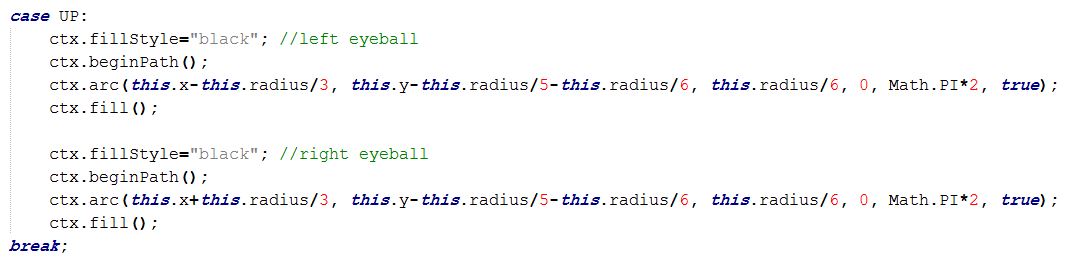
\includegraphics[width=10cm]{pics/Code}
    \label{fig:eyes}
    \end{figure}
\end{frame}

\begin{frame}{Pacman - analysis}
A huge Ghost.draw() function:
 \begin{itemize}
      \item Checks the status of the ghost (weak or strong, moving or not, ..)
      \item Draws every detail (the eyes, mouth, legs, ...)
    \end{itemize}
 \begin{block}{Disadvantages}
      \begin{itemize} 
    \item Hard to understand, to maintain, or to debug.
    \item Repetitive very similar lines of code, no reuse.
    \end{itemize}
    \end{block}
\end{frame}

\begin{frame}[fragile]
\frametitle{Pacman - refactoring}
\textbf{Fa\c{c}ade(s):}
   \begin{itemize}
    \item Re-structured the draw() function by using several helper functions
    \item Reuse of code for drawing eyes at different positions, as well as legs
    \end{itemize}
    \begin{lstlisting}
    
Ghost.prototype.eyeBlack = function (offsetX, offsetY){ ... };

Ghost.prototype.eyeWhite = function (){ ... };

Ghost.prototype.legs = function (){ ... };

Ghost.prototype.mouth = function (){ ... };

\end{lstlisting}
\end{frame}

\begin{frame}[fragile]
\frametitle{Pacman - refactoring}
\textbf{Fa\c{c}ade(s):}
\begin{lstlisting}
Ghost.prototype.eyeBlack = function (offsetX, offsetY){
	ctx.fillStyle="black";
	ctx.beginPath();
	ctx.arc(this.x+offsetX, this.y+offsetY, this.radius/6, 0, Math.PI*2, true); 
	ctx.fill();
};

Ghost.prototype.draw = function (){
...
case UP:
	this.eyeBlack(-this.radius/3, -this.radius/5-this.radius/6);
	this.eyeBlack(this.radius/3, -this.radius/5-this.radius/6);
break;
...
}
\end{lstlisting}
\end{frame}



% Placing a * after \section means it will not show in the
% outline or table of contents.
\section*{Summary}
\begin{frame}{Summary I}
 The decorator pattern:
 \begin{itemize}
\item Objects can be 'decorated' and used with new behavior, without worrying about modifying the base object.
\item Excessive use is not advised, managing them becomes a headache (instantiation of objects, decorators interdependence, ..) 
 \end{itemize}
\end{frame}

\begin{frame}[fragile]
\frametitle{Summary II}
 The proxy pattern:
 \begin{itemize}
\item Introduces a level of indirection that helps in regulating or optimizing access to objects
\item While making access to remote objects completely transparent, inefficient uses can occur
 \end{itemize}
 \begin{lstlisting}
 if (account.getBalance() > 0 && account.getBalance() < MAX) {
    transferAmount(account.getBalance() / 2);
}
 \end{lstlisting}
\end{frame}

\begin{frame}[fragile]
\frametitle{Summary III}
 The fa\c{c}ade pattern:
\begin{itemize}
  \item Promotes decoupling and reuse, enhances structure and maintainability of code.
  \item Need to be aware of the performance costs of the abstraction offered by the fa\c{c}ade
  \end{itemize}
\end{frame}
% All of the following is optional and typically not needed. 

\begin{frame}
  \frametitle{References}    
  \begin{thebibliography}{5}    
  
  \beamertemplatebookbibitems
  \bibitem{stefanov2010}
   Stefanov, S.
    \newblock {\em JavaScript Patterns}.
    \newblock O'Reilly Media, 2010.
  
  \beamertemplatebookbibitems
  \bibitem{osmani2012}
   Osmani, A.
    \newblock {\em Learning JavaScript Design Patterns}.
    \newblock O'Reilly Media, 2012.
  
  \setbeamertemplate{bibliography item}[online]
  \bibitem{A} Sourcemaking
  \newblock {\em Design Patterns Explained Simply}.
  \newblock \url{https://sourcemaking.com/design_patterns}
  
  \setbeamertemplate{bibliography item}[online]
  \bibitem{A} Zaikin, M. 
  \newblock {\em Benefits and Drawbacks of Design Patterns}.
  \newblock \url{http://java.boot.by/scea5-guide/ch07s03.html}
 
  \end{thebibliography}
\end{frame}

\end{document}


